\documentclass{article}

\usepackage[utf8]{inputenc}
\usepackage[T1]{fontenc}
\usepackage[spanish]{babel}
\usepackage{times}
\usepackage{wrapfig}
\usepackage{lmodern}
\usepackage{mathtools}
\usepackage{graphicx}
\usepackage[utf8]{inputenc}
\usepackage{fancyhdr}
\usepackage{color}
\usepackage{hyperref}
\hypersetup{
    colorlinks=true, %set true if you want colored links
    linktoc=all,     %set to all if you want both sections and subsections linked
    linkcolor=blue,  %choose some color if you want links to stand out
}



\definecolor{gray97}{gray}{.97}
\definecolor{gray75}{gray}{.75}
\definecolor{gray45}{gray}{.45}

\usepackage{listings}
  \lstset{ frame=Ltb,
          framerule=0pt,
          aboveskip=0.5cm,
          framextopmargin=3pt,
          framexbottommargin=3pt,
          framexleftmargin=0.4cm,
          framesep=0pt,
          rulesep=.4pt,
          backgroundcolor=\color{gray97},
          rulesepcolor=\color{black},
          %
          stringstyle=\ttfamily,
          showstringspaces = false,
          basicstyle=\small\ttfamily,
          commentstyle=\color{gray45},
          keywordstyle=\bfseries,
          %
          numbers=left,
          numbersep=15pt,
          numberstyle=\tiny,
          numberfirstline = false,
          breaklines=true,
  }

% minimizar fragmentado de listados
\lstnewenvironment{listing}[1][]
  {\lstset{#1}\pagebreak[0]}{\pagebreak[0]}

\lstdefinestyle{consola}{basicstyle=\scriptsize\bf\ttfamily, backgroundcolor=\color{gray75}, }

\lstdefinestyle{C}{language=C,}

\title{Tarea 1.- Creación de la base de datos \textbf{COMPETICIÓN}}
\author{Antonio Muñoz Cubero}
 

\begin{document}
\maketitle
\pagenumbering{gobble}
\pagestyle{fancy} 

\newpage
  \tableofcontents
    \lhead[BD COMPETICION]{BD COMPETICION}
    \lfoot[IES Francisco De Los Rios]{IES Francisco De Los Rios}
      \pagenumbering{roman}

\newpage
  \section{Foto del Modelo Relacional}
    \begin{figure}[h]
      \centering
      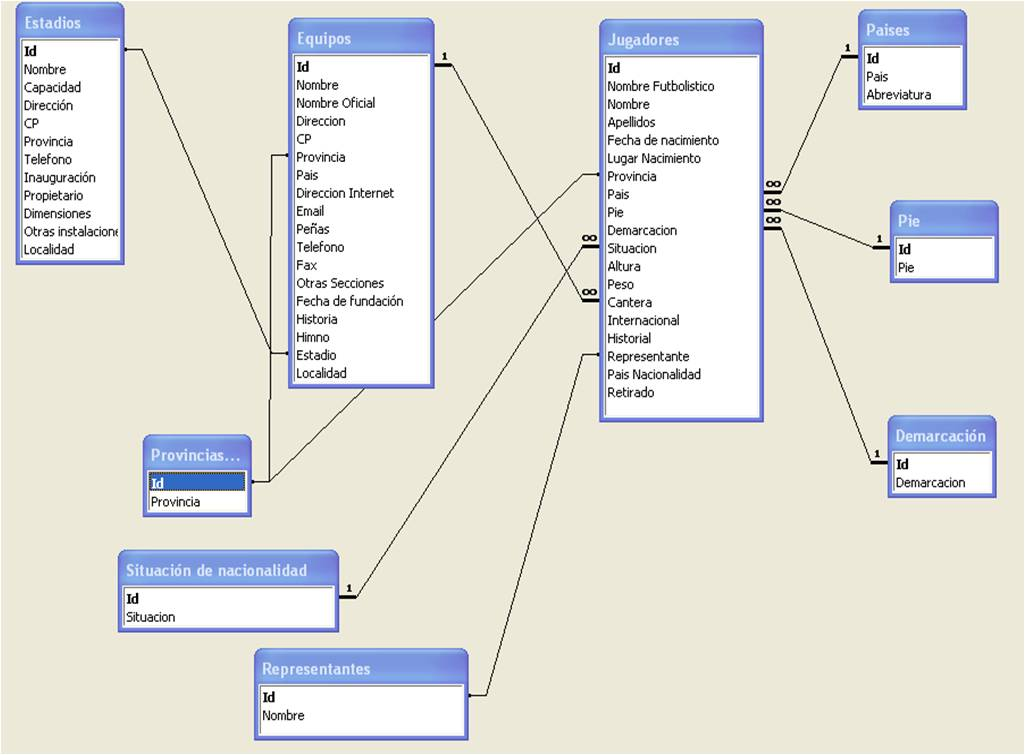
\includegraphics[scale = 0.75]{modelo.jpg}
    \end{figure}
\newpage
  \section{Creación de la Base de Datos}
    Entramos al cliente de MariaDB con el usuario que tengamos para trabjar, acto seguido empezaremos creando 
    la base de datos \textbf{competicion} usando los siguientes comandos, después la seleccionamos y comenzamos la creación de las tablas. 
    \begin{listing}[style=consola, numbers=none]
    MariaDB [(none)]> CREATE DATABASE IF NOT EXISTS competicion;

    MariaDB [(none)]> USE competicion;

    \end{listing}
  \section{Creación de las tablas}
    En este caso, las tablas debemos de comenzar a crearlas teniendo en cuenta si hay claves que dependan de otras o no, en nuestro caso, empezaremos creando 
    la taba \textbf{estadio}, que no depende de ninguna y posteriormente la tabla \textbf{provincia}.
    \subsection{Tabla 'estadio'}
      \begin{lstlisting}[style=C]
        CREATE TABLE IF NOT EXISTS estadio(
          idEstadio INT(5) NOT NULL AUTO_INCREMENT,
          nombre VARCHAR(50) NOT NULL,
          capacidad INT(17) NOT NULL,
          direccion VARCHAR(50),
          cp INT(5) NOT NULL,
          provincia VARCHAR(20) NOT NULL,
          telefono INT(9) NOT NULL,
          inauguracion DATE NOT NULL,
          propietario VARCHAR(50) NOT NULL,
          dimensiones INT(10) NOT NULL,
          otrasInstalaciones VARCHAR(50),
          localidad VARCHAR(20) NOT NULL,
          CONSTRAINT pk_estadio_idEstadio PRIMARY KEY (idEstadio),
          CONSTRAINT u_estadio_telefono UNIQUE (telefono),
          CONSTRAINT u_estadio_direccion UNIQUE (direccion)
        )
        ENGINE = InnoDB
        COMMENT ='Tabla donde se definen los estadios que existen.'
        ;
      \end{lstlisting}
\newpage
   \subsection{Tabla 'provincia'}   
    \begin{lstlisting}[style=C]
      CREATE TABLE IF NOT EXISTS provincia(
        idProvincia INT(5) NOT NULL AUTO_INCREMENT,
        provincia VARCHAR(20) NOT NULL,
        CONSTRAINT pk_provincia_idProvincia PRIMARY KEY (idProvincia)
      )
      ENGINE = InnoDB
      COMMENT ='Tabla donde se definen las provincias que existen. que son referidas en varias tablas'
      ;
    \end{lstlisting}
\newpage
  Ahora creamos la tabla \textbf{equipo}, la cual hace referencia a \textbf{estadio} y \textbf{provincia} creadas 
  anteriormente, por lo cual, no habrá error.
  \subsection{Tabla 'equipo'}
    \begin{lstlisting}[style=C]
      CREATE TABLE IF NOT EXISTS equipo(
        idEquipo INT(5) NOT NULL AUTO_INCREMENT,
        nombre VARCHAR(50) NOT NULL,
        nombreOficial VARCHAR(50) NOT NULL,
        direccion VARCHAR (50) NOT NULL,
        cp INT(5) NOT NULL,
        idProvincia INT(5) NOT NULL,
        pais VARCHAR(20) NOT NULL,
        direccionInternet VARCHAR(20) NOT NULL,
        email VARCHAR(20) NOT NULL,
        penias VARCHAR(20) NOT NULL,
        telefono INT(9) NOT NULL,
        fax INT(9) NOT NULL,
        otrasSecciones VARCHAR(20),
        fechaFundacion DATE NOT NULL,
        historia VARCHAR(20) NOT NULL,
        himno VARCHAR(20) NOT NULL,
        idEstadio INT(5) NOT NULL,
        localidad VARCHAR(20) NOT NULL,
        CONSTRAINT pk_equipo_idEquipo PRIMARY KEY (idEquipo),
        CONSTRAINT fk_equipo_idProvincia FOREIGN KEY (idProvincia) REFERENCES provincia (idProvincia),
        CONSTRAINT fk_equipo_idEstadio FOREIGN KEY (idEstadio) REFERENCES estadio (idEstadio),
        CONSTRAINT u_equipo_telefono UNIQUE (telefono),
        CONSTRAINT u_equipo_email UNIQUE (email),
        CONSTRAINT u_equipo_fax UNIQUE (fax),
        CONSTRAINT u_equipo_nombreOficial UNIQUE (nombreOficial)
      )
      ENGINE = InnoDB
      COMMENT = 'Tabla donde almacenamos los datos de los equipos.'
      ;
    \end{lstlisting}
\newpage
  Ahora creamos todas las tablas a las que la tablas \textbf{jugador}, que crearemos la última, hace referencia.
  \subsection{Tabla representante}  
    \begin{listing}[style=C]
      CREATE TABLE IF NOT EXISTS representante( 
        idRepresentante INT(5) NOT NULL AUTO_INCREMENT,
        nombre VARCHAR(20) NOT NULL,
        CONSTRAINT pk_provincia_idRepresentante PRIMARY KEY (idRepresentante)
      )
      ENGINE = InnoDB
      COMMENT ='Tabla donde se definen los representantes que existen. que son referidas en varias tablas'
      ;
    \end{listing}
  \subsection{Tabla 'demarcacion'}
    \begin{listing}[style=C]
      CREATE TABLE IF NOT EXISTS demarcacion(
        idDemarcacion INT(5) NOT NULL AUTO_INCREMENT,
        demarcacion VARCHAR(20) NOT NULL,
        CONSTRAINT pk_provincia_idDemarcacion PRIMARY KEY (idDemarcacion),
        CONSTRAINT u_demarcacion_demarcacion UNIQUE (demarcacion)
      )
      ENGINE = InnoDB
      COMMENT ='Tabla donde se definen las demarcaciones que existen. que son referidas en varias tablas'
      ;
    \end{listing}
  \subsection{Tabla 'pie'}
    \begin{listing}[style=C]
      CREATE TABLE IF NOT EXISTS pie(
        idPie INT(5) NOT NULL AUTO_INCREMENT,
        pie VARCHAR(20) NOT NULL,
        CONSTRAINT pk_provincia_idPie PRIMARY KEY (idPie)
      )
      ENGINE = InnoDB
      COMMENT ='Tabla donde se definen  que existen. que son referidas en varias tablas'
      ;
    \end{listing}

  \newpage
  \subsection{Tabla 'pais'}
    \begin{listing}[style=C]
      CREATE TABLE IF NOT EXISTS pais(
        idPais INT(5) NOT NULL AUTO_INCREMENT,
        pais VARCHAR(20) NOT NULL,
        abreviatura VARCHAR(5) NOT NULL,
        CONSTRAINT pk_provincia_idPie PRIMARY KEY (idPais),
        CONSTRAINT u_pais_pais UNIQUE (pais),
        CONSTRAINT u_pais_abreviatura UNIQUE (abreviatura)
      )
      ENGINE = InnoDB
      COMMENT ='Tabla donde se definen los paises que existen. que son referidas en varias tablas'
      ;
    \end{listing}
  \subsection{Tabla 'situacionNacionalidad'}
    \begin{listing}[style=C]
      CREATE TABLE IF NOT EXISTS situacionNacionalidad(
        idSituacionNacionalidad INT(5) NOT NULL AUTO_INCREMENT,
        situacion VARCHAR(20) NOT NULL,
        CONSTRAINT pk_provincia_idSituacionNacionalidad PRIMARY KEY (idSituacionNacionalidad)
      )
      ENGINE = InnoDB
      COMMENT ='Tabla donde se definen las situaciones de nacionalidad que existen. que son referidas en varias tablas'
      ;
    \end{listing}
  
  Por último con respecto a la creación de las tablas de la base de datos \textbf{competicion}, creamos la tabla \textbf{jugador}, la cual hace referencia a la mayoria 
  de tablas creadas anteriormente, por ello, es la último que creo.

\newpage
  \subsection{Tabla 'jugador'}
    \begin{listing}[style=C]
      CREATE TABLE IF NOT EXISTS jugador(
        idJugador INT(5) NOT NULL AUTO_INCREMENT,
        nombreFutbolistico VARCHAR(10) NOT NULL,
        nombre VARCHAR(10) NOT NULL,
        apellidos VARCHAR(20) NOT NULL,
        fechaNacimiento DATE NOT NULL,
        lugarNacimiento VARCHAR(20) NOT NULL,
        idProvincia INT(5) NOT NULL,
        idPais INT(5) NOT NULL,
        idPie INT(5) NOT NULL,
        idDemarcacion INT(5) NOT NULL,
        idSituacionNacionalidad INT(5) NOT NULL,
        altura INT(10) NOT NULL,
        peso INT(10) NOT NULL,
        idEquipo INT(5) NOT NULL,
        internacional BOOLEAN NOT NULL,
        historial VARCHAR(20) NOT NULL,
        idRepresentante INT(5) NOT NULL,
        paisNacionalidad VARCHAR(15) NOT NULL,
        retirado BOOLEAN NOT NULL,
        CONSTRAINT pk_jugador_idJugador PRIMARY KEY (idJugador),
        CONSTRAINT fk_jugador_idProvincia FOREIGN KEY (idProvincia) REFERENCES provincia (idProvincia),
        CONSTRAINT fk_jugador_idPais FOREIGN KEY (idPais) REFERENCES pais (idPais),
        CONSTRAINT fk_jugador_idPie FOREIGN KEY (idPie) REFERENCES pie (idPie),
        CONSTRAINT fk_jugador_idDemarcacion FOREIGN KEY (idDemarcacion) REFERENCES demarcacion (idDemarcacion),
        CONSTRAINT fk_jugador_idSituacionNacionalidad FOREIGN KEY (idSituacionNacionalidad) REFERENCES situacionNacionalidad (idSituacionNacionalidad),
        CONSTRAINT fk_jugador_idEquipo FOREIGN KEY (idEquipo) REFERENCES equipo (idEquipo),
        CONSTRAINT fk_jugador_idRepresentante FOREIGN KEY (idRepresentante) REFERENCES representante (idRepresentante)
      )
      ENGINE = InnoDB
      COMMENT ='Tabla donde se definen los jugadores que existen.'
      ;
    \end{listing}
\newpage
  \section{Modelo Relacional}
    En mi caso la creación de la base de datos \textbf{competicion}, en una primera instancia la hice en \textit{Windows10} con el cliente de \textbf{MySQL}, 
    después de que la implementación fuese correcta, exporté el archivo .sql desde \textit{HeidiSQL}. Una vez en \textit{Linux(ubuntu 20.04 LTS)} importé la 
    base de datos y con gran éxito pude visializarla en el programa \textbf{DBeaver}, una vez dentro del programa, pude visualizar sin problema el \textbf{modelo relacional}.

    \begin{figure}[h]
      \centering
      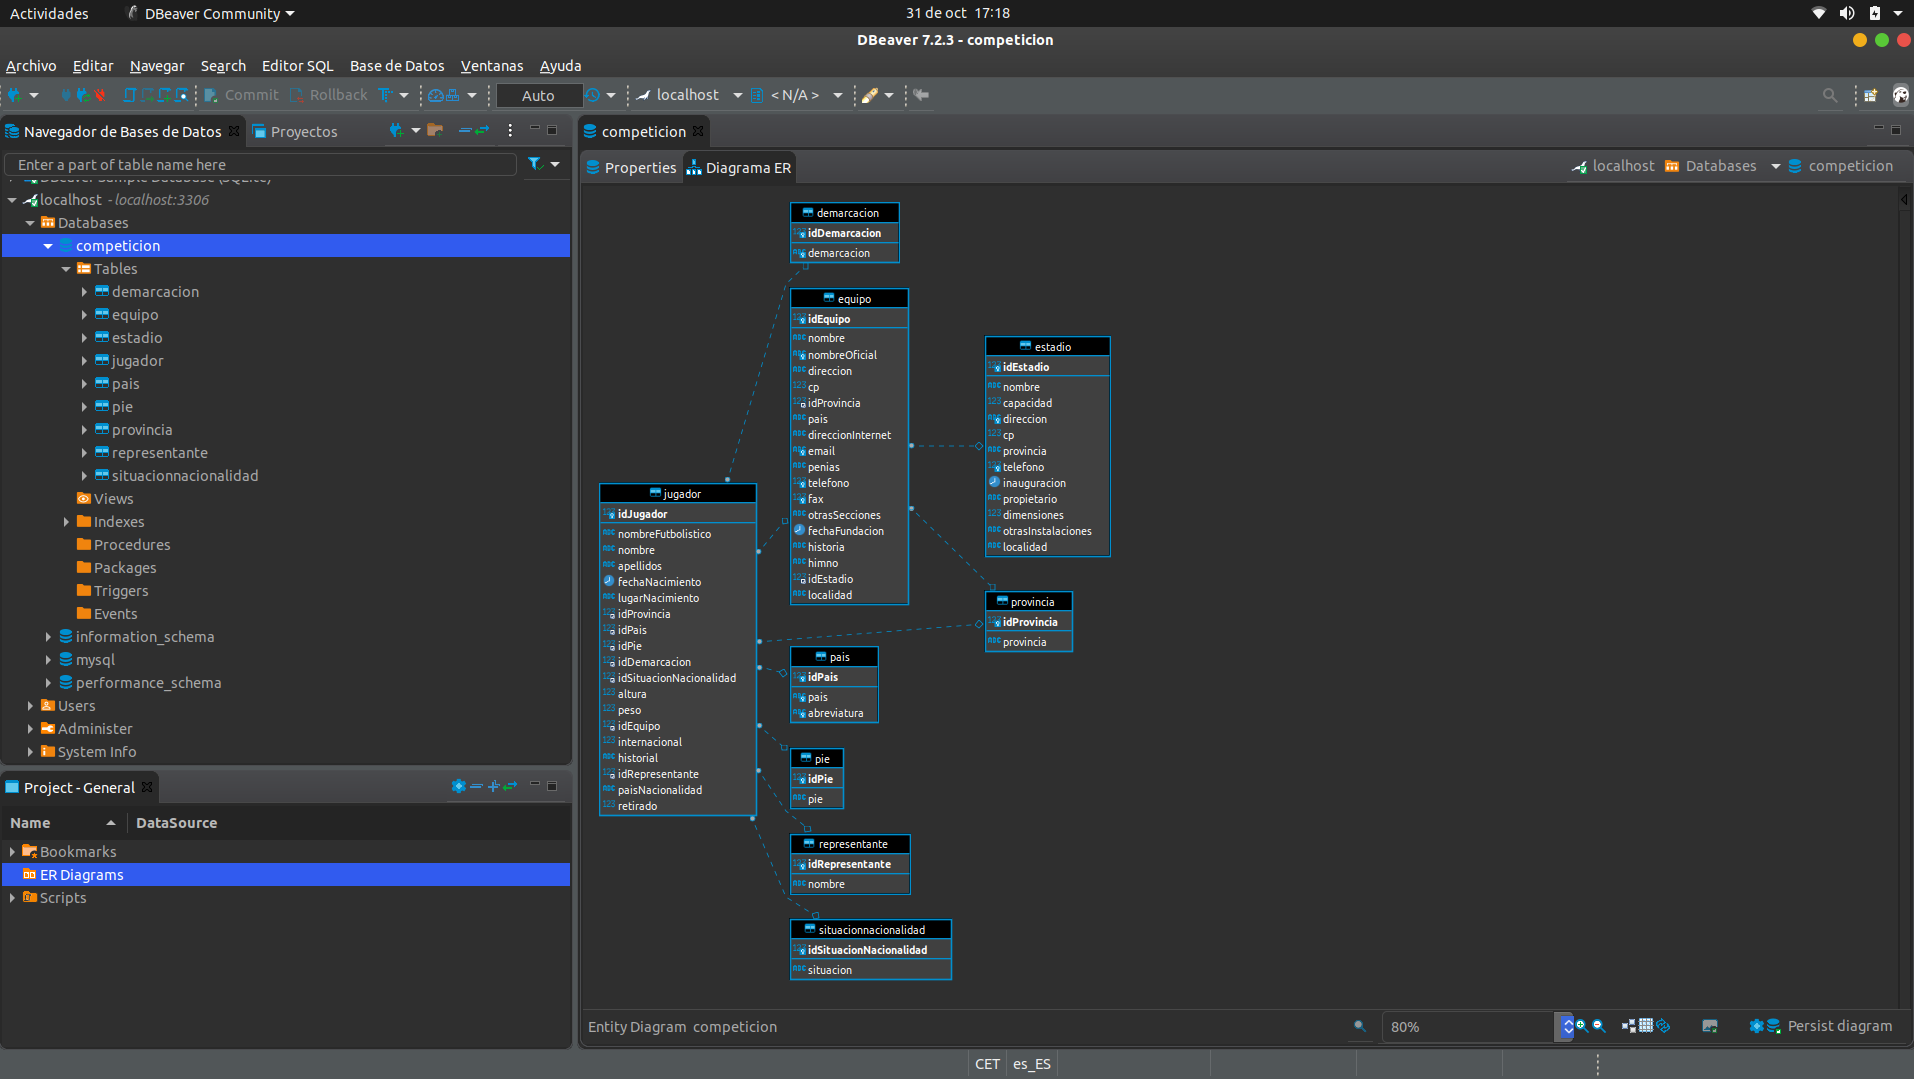
\includegraphics[scale = 0.183]{entidad-relacion_competicion.png}
    \end{figure}

\newpage
  \section{Aclaraciones}
    En la carpeta de la entrega, como se puede observar, tengo varios archivos \textit{.sql}, el primer archivo \textbf{competicion-dbeaver.sql} es el resultado de exportar la base de datos
    \textit{competicion} en el programa \textbf{Dbeaver}.
    \\\\
    El archivo \textbf{competicion-heidi.sql} es el archivo resultante de la exportación de la base de datos desde el programa \textit{HeidiSQL}.
    \\\\
    El archivo \textbf{competicion-sucio.sql} es el archivo que yo he creado para la primera implementación de la base de datos \textbf{competicion}, de la cual exporté los demás archivos. Es el archivo primigenio.
\end{document}